Fig. 3 shows the architecture of \textit{Apache Openwhisk}, which consists of two primary components: the \textbf{Controller} and the \textbf{Invoker}, built on \textbf{Nginx}, \textbf{Kafka}, \textbf{Docker}, and \textbf{CouchDB}. Together, these components enable OpenWhisk to function as a \textit{serverless event-driven programming service}. OpenWhisk offers a \textit{RESTful API} that allows users to submit functions and retrieve execution results.\vspace{10pt}
\begin{center}
    \includegraphics[width=0.6\textwidth]{img/ow_arch.png}
    \captionof{figure}{Apache Openwhisk architecture}
    \vspace{10pt}
\end{center}
\textbf{Nginx} routes incoming requests to the \textit{Controller}, which handles authentication, retrieves the requested functions from the \textbf{CouchDB} database, and directs them to the \textit{Invokers} acting as a \textit{Load Balancer}.\vspace{14pt}\\
\textbf{Kafka}, a high-performance message distribution system, facilitates communication between the \textit{Controller} and the \textit{Invokers}.\vspace{14pt}\\
The \textit{Invokers}, distributed across multiple machines and responsible for hosting serverless function containers, execute function calls by allocating resources within \textbf{Docker} containers and assigning a container to each function invocation. Essentially, \textit{Invokers} serve as the \textit{worker nodes} in Openwhisk (as represented in Fig. 1).\vspace{14pt}\\
Each \textit{Invoker} has an in-memory queue to manage function requests when resources are temporarily unavailable. Once resources are freed, functions are dequeued and executed in a \textbf{First Come First Serve} (\textbf{FCFS}) order. All \textit{Invokers} use the same instructions embedded in the \textit{Invoker component's source code} (written in \textit{Scala}), ensuring uniform operation across all \textit{Invokers}.\vspace{14pt}\\
Users can register on the platform to upload their functions, specifying only the memory required for each function's execution.\cite{banaei2022etas}\vspace{14pt}\\
Fig. 4 shows how Openwhisk processes an action into more details.\cite{sciabarra2019learning}\vspace{10pt}
\begin{center}
    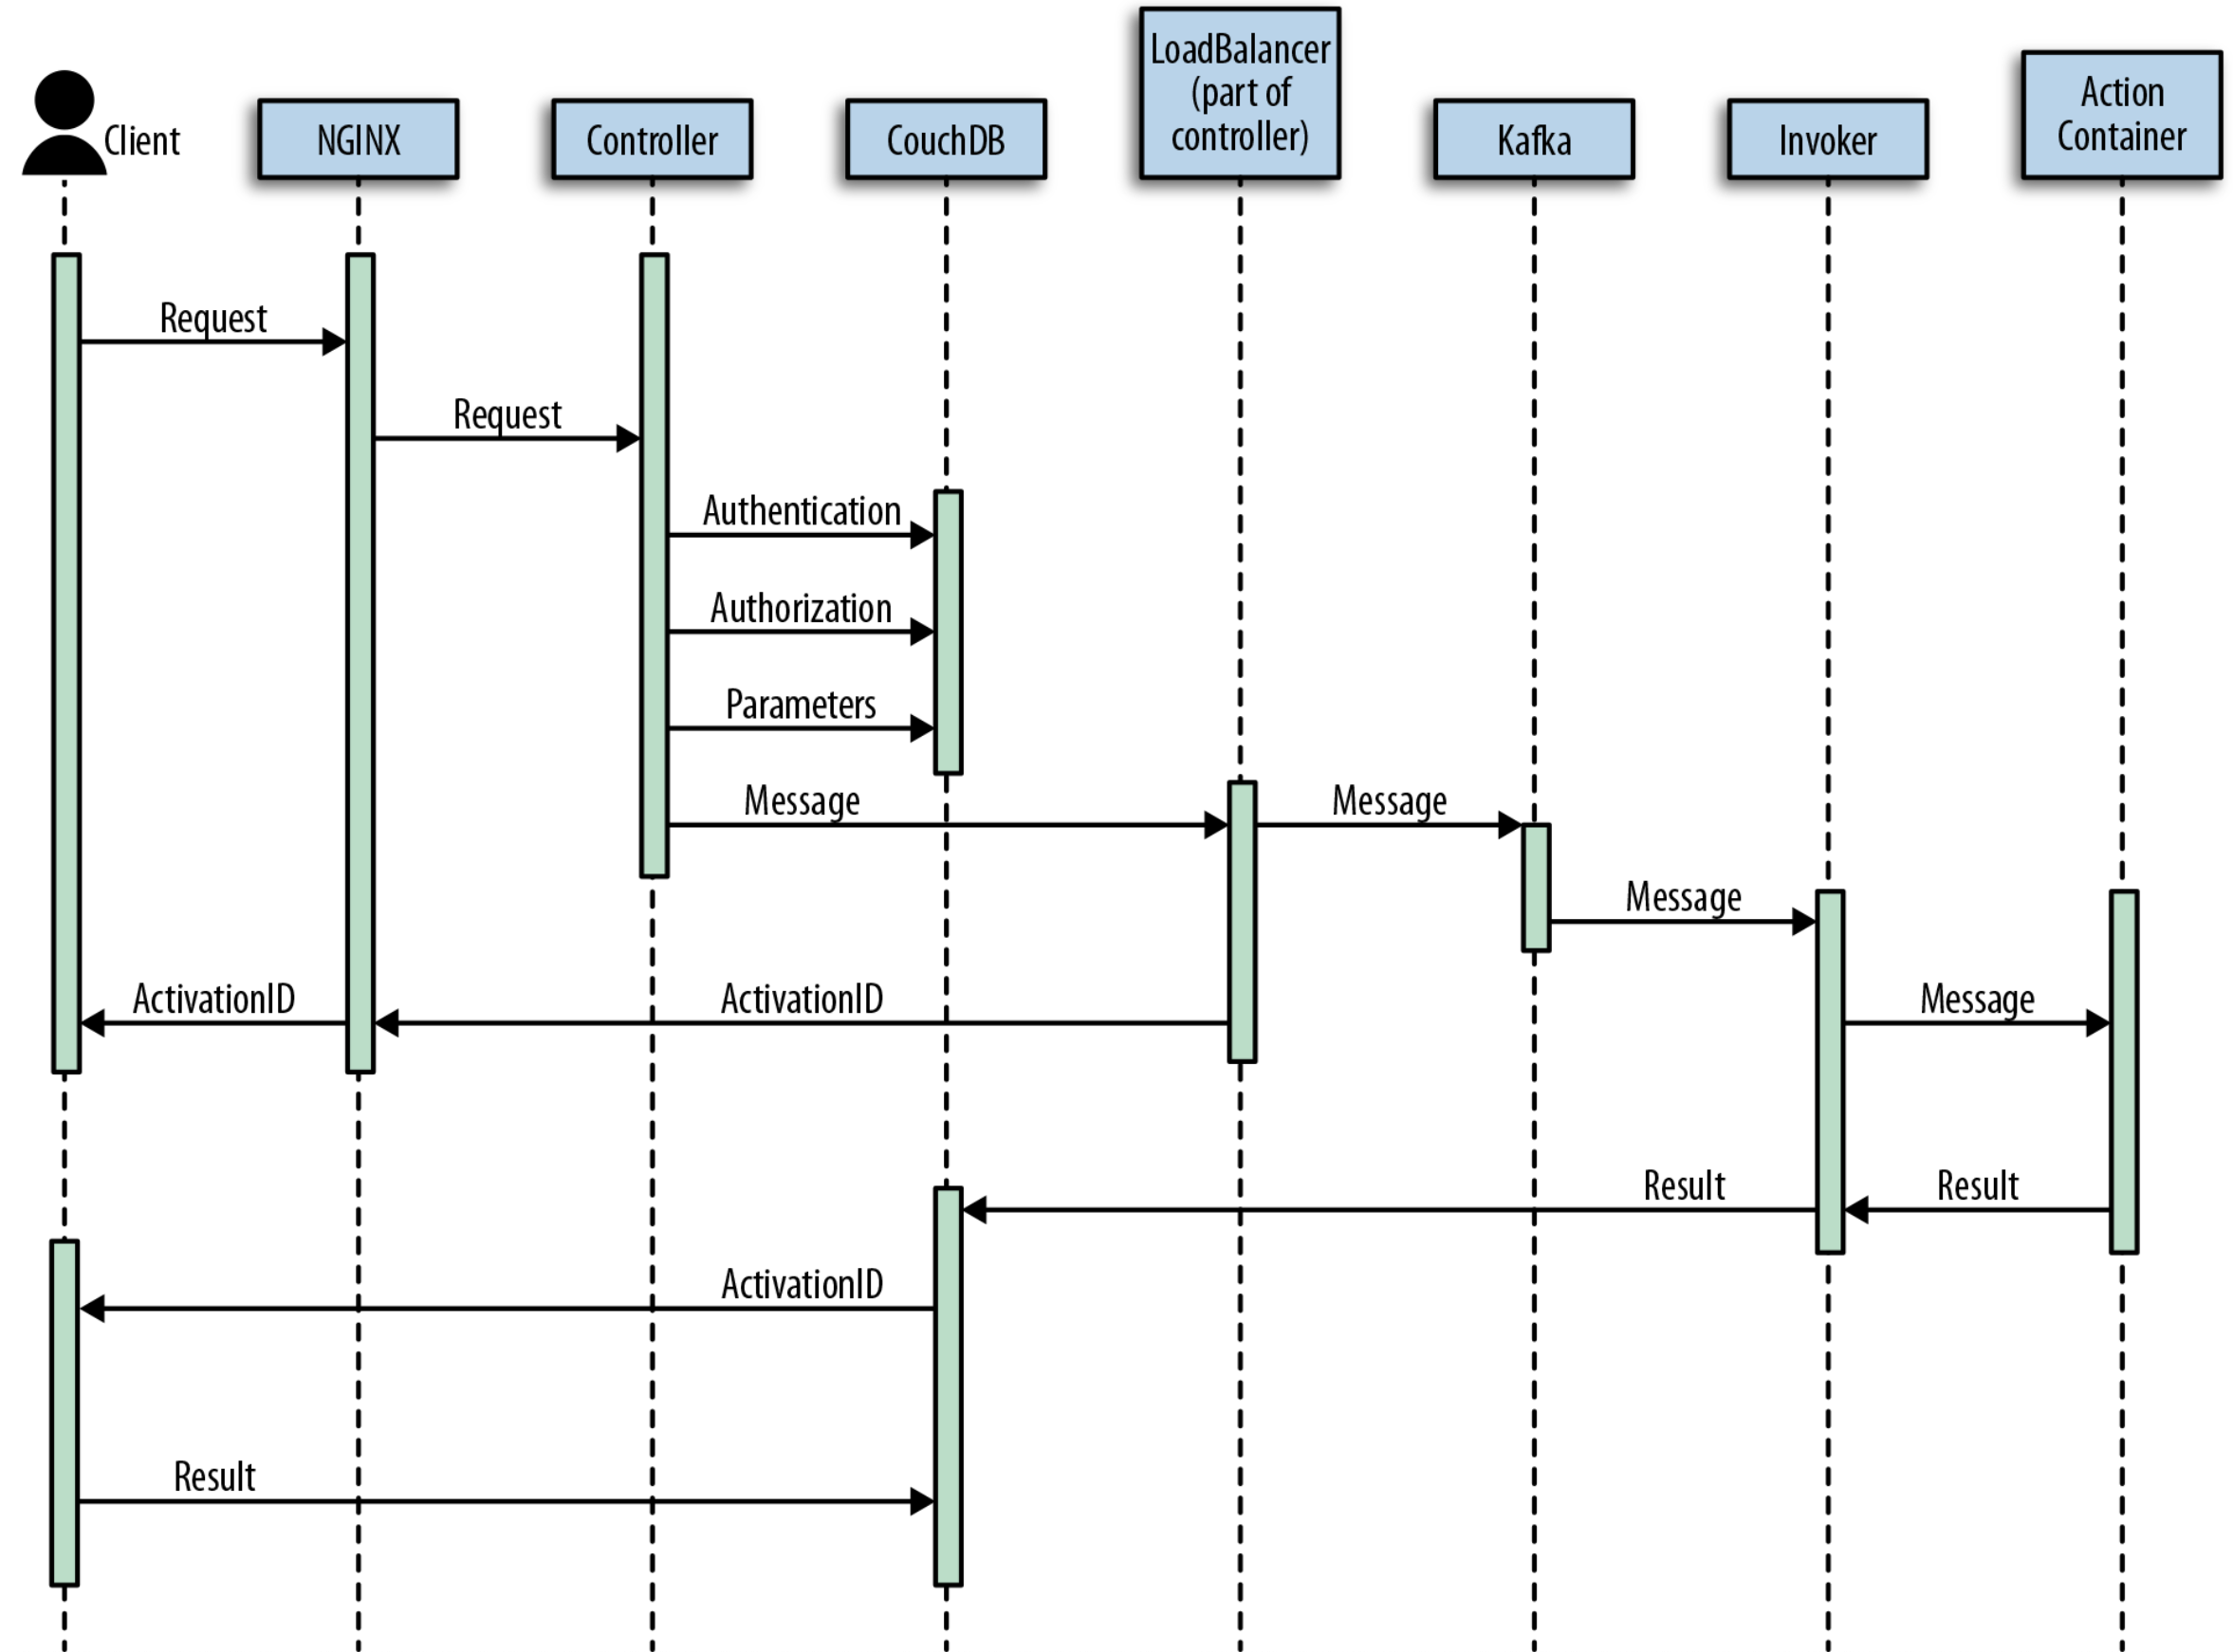
\includegraphics[width=0.95\textwidth]{img/sequence.png}
    \captionof{figure}{How OpenWhisk processes an action}
    \vspace{10pt}
\end{center}
\textbf{Nginx}\\
The process begins when an action is invoked, which can happen in several ways:
\begin{itemize}
    \item Via the web, if the action is set up as a web-accessible action.
    \item Through the API, when one action calls another.
    \item By activating a trigger with a rule linked to the action.
    \item From the CLI (Command Line Interface).
\end{itemize}
The "client" refers to the entity initiating the action. As OpenWhisk is a RESTful system, each invocation is translated into an HTTPS request that first reaches the "edge" node. This edge node is the web server and reverse proxy, Nginx. Nginx’s primary function here is to handle HTTPS, deploying the necessary certificates for secure processing.\\
Once secure, Nginx forwards the request to the system's core service component, the controller.\vspace{14pt}\\
\textbf{Controller}\\
Before executing an action, the controller verifies that the action can be properly executed and initialized:
\begin{itemize}
    \item \textbf{Authentication}: the controller must first authenticate the request to confirm it can execute the action.
    \item \textbf{Authorization}: after confirming the request’s origin, the controller checks that the client has the necessary permissions to proceed.
    \item \textbf{Parameter Enrichment}: the request is then supplemented with additional parameters that are part of the action’s configuration.
\end{itemize}
To carry out these steps, the controller consults CouchDB, the database used by OpenWhisk. Once the request is validated and enriched, the action is ready for execution and is sent to the load balancer, the next step in the processing flow.\vspace{14pt}\\
\textbf{Load Balancer}\\
The load balancer in OpenWhisk is responsible for distributing the processing load across various executors, known as invokers.\\
Since OpenWhisk runs actions within designated runtimes, the load balancer tracks available runtime instances. When possible, it reuses existing instances to execute actions; if not, it creates new instances as needed.\vspace{14pt}\\
When the system is ready to invoke an action, the load balancer can't send requests directly to an invoker if it is already occupied, has crashed, or if the system is undergoing a restart. Operating in a highly parallel, scalable environment means the system may not always have immediate resources available, necessitating a buffer for pending invocations. OpenWhisk uses Kafka for this buffering.\vspace{14pt}\\
Kafka, a high-performance "publish and subscribe" messaging system, stores requests until they are ready for execution. Each action invocation is converted into an HTTPS request to Nginx, which is then transformed into a Kafka message directed to the chosen invoker.\\
Each message assigned to an invoker includes a unique identifier, the activation ID. Once queued in Kafka, the system offers two types of invocation responses:
\begin{itemize}
    \item \textbf{Nonblocking Invocation}: the activation ID is immediately returned to the client as the response, completing the request. The client can later use this ID to retrieve the invocation result.
    \item \textbf{Blocking Invocation}: the connection remains open as the controller waits for the action to complete. Once the result is ready, it is sent directly to the client.
\end{itemize}
\vspace{5pt}
\textbf{Invoker}\\
In OpenWhisk, the invoker is responsible for executing actions within isolated environments provided by Docker containers. Docker containers simulate a complete operating system, offering a self-contained environment with all dependencies needed to run an action.\vspace{14pt}\\
From the action’s viewpoint, the Docker container resembles a full computer, similar to a virtual machine (VM), but container execution is significantly more efficient than VMs, making containers the preferred choice.\\
Docker uses images to create containers for action execution. Each runtime corresponds to a Docker image, and the invoker launches a new image for the specified runtime, then loads the action’s code into it. OpenWhisk offers a variety of pre-built Docker images that support different programming languages, including JavaScript, Python, Go, and Java. These images come with initialization logic specific to each runtime.\\
Once the runtime environment is initialized, the invoker processes action requests, handling and storing logs to aid debugging.\vspace{14pt}\\
After the action execution is complete, OpenWhisk stores the result in CouchDB (also used for configuration data storage). Each action result is tagged with the activation ID, which was previously provided to the client. This allows the client to retrieve the execution result later by querying CouchDB using the activation ID.\vspace{14pt}\\
\textbf{Client}\\
The processing flow in OpenWhisk is primarily asynchronous. In this mode, the client initiates a request and receives an activation ID, which acts as a reference for the invocation. This activation ID allows OpenWhisk to store the result of the action in the database upon completion. To retrieve the final result, the client must send another request later, using the activation ID as a parameter. Once the action finishes, the result, logs, and additional information are stored in the database, making them accessible for the client.\vspace{14pt}\\
OpenWhisk also supports synchronous processing, which operates similarly but with one key difference: the client’s request remains open, blocking until the action completes, allowing the client to immediately receive the result.\cite{sciabarra2019learning}